%%%%%%%%%%%%%%%%%%%%%%%%%%%%%%%%%%%%%%%%%%%%%%%%%%%%%%%%%%%%%%%%%%%%%%
% Lớp 11 | Quan hệ vuông góc trong không gian | Đường thẳng vuông góc với mặt phẳng
% Dạng 1H8?2-4: Dựng mặt phẳng, tìm thiết diện
% Số câu: 14  (sinh tự động bởi tach_cau.py; từ nay thầy sửa trực tiếp file này)
%%%%%%%%%%%%%%%%%%%%%%%%%%%%%%%%%%%%%%%%%%%%%%%%%%%%%%%%%%%%%%%%%%%%%%

%%%%%%%%%%%%%%%% TRẮC NGHIỆM 4 PHƯƠNG ÁN %%%%%%%%%%%%%%%%

% nguồn: Ok_Toan11_TracNghiem_Lan2
\begin{ex}%[1H8H2-4]%[ma:a957f039]
	Cho hình lập phương $ABCD.A'B'C'D'$. Thiết diện của  hình lập phương cắt bởi mặt phẳng $(\alpha)$ qua $C$ và vuông góc $BD$ là hình gì?
	 \choice
		{Ngũ  giác}
		{\True Hình chữ nhật} 
		{Hình vuông} 
		 {Tam giác cân}
	 \loigiai{
		\begin{center}
			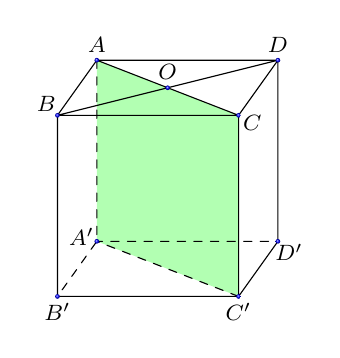
\begin{tikzpicture}[scale=1,>=stealth,font=\footnotesize,line join=round,line cap=round,declare function={h=2.3;}]
					 \path
						(0,0) coordinate (A) 
						 (-0.5,-0.7) coordinate (B)
						(B)+(0:h) coordinate  (C)
						(barycentric cs:A=1,C=1,B=-1) coordinate (D) 
						(A)+(-90:h) coordinate (A') 
						(barycentric cs:A=-1,B=1,A'=1)  coordinate (B')
						 (barycentric cs:A=-1,C=1,A'=1) coordinate (C')
						(barycentric cs:A=-1,D=1,A'=1) coordinate  (D')
						(intersection of A--C and  B--D) coordinate (O);
					\fill[green!30]  (A)--(C)--(C')--(A')--cycle;
					\draw[dashed]  (A)--(A')--(B')
						 (C')--(A')--(D');
					 \draw (D)--(A)--(B)--(B')--(C')--(D')--(D)--(C)--(B)--(D)
						 (A)--(C)--(C');
					\foreach \p/\g in{A'/165,B'/-90,C'/-90,D'/-45,A/90,B/135,C/-30,D/90,O/90} 
					\shade[shading=ball](\p) circle (.03) node[shift={(\g:.2)},scale=1]{$\p$}; 
				\end{tikzpicture}
		\end{center}
		Ta có  $CA\perp BD$ và $CC'\perp BD$ suy ra $(ACC'A')\perp BD$.\\
		Vì vậy $(\alpha)$ chính là  $(ACC'A')$. Thiết diện là một hình chữ nhật $ACC'A'$.\\
		Hơn nữa, $AC>CC'$ nên $ACC'A'$ không phải  là hình vuông.
	} 
\end{ex}

% nguồn: Ok_Toan11_TracNghiem_Lan2
\begin{ex}%[1H8V2-4]%[ma:a8e7a090]
	Cho hình hộp  chữ nhật $ABCD.A'B'C'D'$ có $AB=a$, $AD=2a$, $AA'=a\sqrt{2}$. Tính diện tích của thiết diện của hình hộp chữ nhật khi được cắt bởi mặt phẳng $(\alpha)$ qua $A$ và vuông góc $A'B$.
	 \choice
		{$\dfrac{a^2\sqrt{3}}{2}$} 
		{$2a^2$} 
		 {$a^2\sqrt{2}$}
		 {\True $a^2\sqrt{6}$}
	\loigiai{ 
		\begin{center}
			\begin{tikzpicture}[scale=1,>=stealth,font=\footnotesize,line join=round,line cap=round,declare function={h=2.3; k=h*sqrt (2);}]
					 \path
						 (0,0) coordinate (A)
						(-0.5,-0.7) coordinate (B) 
						(B)+(0:k) coordinate (C) 
						(barycentric  cs:A=1,C=1,B=-1) coordinate (D)
						 (A)+(-90:h) coordinate (A')
						(barycentric cs:A=-1,B=1,A'=1)  coordinate (B')
						(barycentric cs:A=-1,C=1,A'=1) coordinate (C') 
						(barycentric  cs:A=-1,D=1,A'=1) coordinate (D')
						(barycentric cs:B'=1,B=1) coordinate (M) 
						(barycentric cs:C'=1,C=1)  coordinate (N)
						 (intersection of A--M and B--A') coordinate (E);
					 \draw[dashed] (M)--(A)--(A')--(B')
						 (B)--(A')--(D');
					 \draw (M)--(N)--(D)--(A)--(B)--(B')--(C')--(D')--(D)--(C)--(B)
						 (C)--(C');
					 \pic[draw,angle radius=3]{right angle=A'--E--M};
					\foreach \p/\g  in{A'/-45,B'/-90,C'/-90,D'/-45,A/90,B/135,C/120,D/90,M/180,N/-10,E/-10}
					\fill (\p) circle (.03) node[shift={(\g:.2)},scale=1]{$\p$}; 
				\end{tikzpicture}
			 \hspace{2cm}
			\begin{tikzpicture}[scale=1,>=stealth,font=\footnotesize,line join=round,line cap=round,declare function={h=2.3; l=h/sqrt (2);}]
					\path 
						(0,0) coordinate  (A)
						 (A)+(180:l) coordinate (B)
						(A)+(-90:h) coordinate (A') 
						(barycentric  cs:A=-1,B=1,A'=1) coordinate (B')
						(barycentric cs:B'=1,B=1)  coordinate (M)
						(intersection of A--M and B--A')  coordinate (E);
					 \draw (M)--(A)--(B)--(B')--(A')--(A)
						(A')--(B)--(B'); 
					\draw[->](A)--+(0:0.7)  node[shift={(-110:.2)}]{$x$};
					 \draw[->](A)--+(90:0.7) node[shift={(220:.2)}]{$y$};
					\pic[draw,angle radius=3]{right  angle=A'--E--M};
					\foreach \p/\g  in{A'/-45,B'/-90,A/135,B/135,M/180,E/-10}
					\fill  (\p) circle (.03) node[shift={(\g:.2)},scale=1]{$\p$};
				\end{tikzpicture}
		\end{center}
		Gọi $M$ là  trung điểm $BB'$.\\
		Xét  mặt phẳng tọa độ $Oxy$ sao cho tia $Ox$ là tia đối của tia $AB$, tia $Oy$ là tia đối của tia $AA'$, đơn vị trên trục là $a$.\\
		Khi  đó, $A(0;0)$, $B(-1;0)$, $A'\left(0;-\sqrt{2}\right)$, $B'\left(-1;-\sqrt{2}\right)$, $M\left(-1;-\dfrac{\sqrt{2}}{2}\right)$.\\
		Ta  có $\vec{AM}=\left(-1;-\dfrac{\sqrt{2}}{2}\right)$, $\vec{A'B}=\left(-1;\sqrt{2}\right)$.\\
		Ta có $\vec{AM}\cdot\vec{A'B}=0$ nên $AM\perp  A'B$.\\
		Ta lại có $AD\perp A'B$.  Suy ra $(\alpha)$ chính là $(ADM)$.\\
		Qua $M$ kẻ $MN\parallel AD$ $(N\in CC')$. Thiết  diện khi đó là hình chữ nhật $ADNM$.\\
		Ta  tính được $AM=\dfrac{a\sqrt{6}}{2}$ và $AD=2a$. Suy ra diện tích hình chữ nhật $ADNM$ là $a^2\sqrt{6}$.
	} 
\end{ex}

% nguồn: Ok_Toan11_TracNghiem_Lan2
\begin{ex}%[1H8V2-4]%[ma:2d50dcea]
	Cho hình lập phương $ABCD.A'B'C'D'$ có cạnh bằng  $a$. Cắt hình lập phương bởi mặt phẳng trung trục của $BD'$. Diện tích thiết diện tạo thành bằng
	 \choice
		{\True  $\dfrac{3a^2\sqrt{3}}{4}$}
		{$\dfrac{a^2\sqrt{3}}{2}$} 
		{$a^2\sqrt{2}$} 
		 {$\dfrac{a^2\sqrt{3}}{4}$}
	 \loigiai{
		\begin{center}
			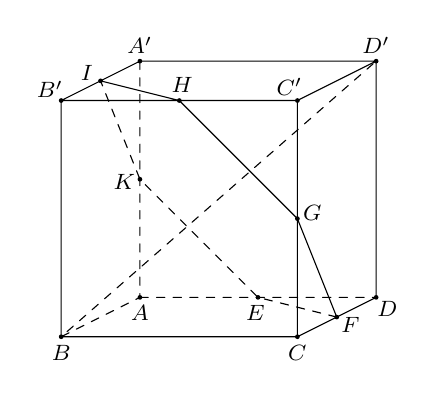
\begin{tikzpicture}[scale=1,>=stealth,font=\footnotesize,line join=round,line cap=round,declare function={h=3;}]
					\path 
						(0,0) coordinate  (A)
						(-1,-0.5) coordinate (B) 
						 (B)+(0:h) coordinate (C)
						 (barycentric cs:A=1,C=1,B=-1) coordinate (D)
						(A)+(90:h)  coordinate (A')
						(barycentric cs:A=-1,B=1,A'=1) coordinate (B') 
						(barycentric cs:A=-1,C=1,A'=1)  coordinate (C')
						(barycentric  cs:A=-1,D=1,A'=1) coordinate (D')
						(barycentric cs:A=1,D=1) coordinate (E) 
						(barycentric cs:C=1,D=1)  coordinate (F)
						(barycentric cs:C=1,C'=1) coordinate  (G)
						 (barycentric cs:B'=1,C'=1) coordinate (H)
						 (barycentric cs:A'=1,B'=1) coordinate (I)
						 (barycentric cs:A=1,A'=1) coordinate (K);
					\draw[dashed] (A')--(A)--(B)--(D') 
						 (A)--(D)
						(F)--(E)--(K)--(I); 
					\draw (D')--(A')--(B')--(B)--(C)--(D)--(D')--(C')--(B') 
						 (C)--(C')
						 (F)--(G)--(H)--(I);
					 \foreach \p/\u in{A/-90,B/-90,C/-90,D/-45,A'/90,B'/135,C'/120,D'/90,E/-100,F/-30,G/20,H/80,I/150,K/190}
					 \fill (\p) circle (.03) node[shift={(\u:.2)},scale=1]{$\p$};
				\end{tikzpicture}
		\end{center}
		Gọi $E$ là trung điểm của $AD$. Ta có $EB=ED'$ nên  $E$ thuộc mặt phẳng trung trực của $BD'$.\\
		Gọi $F$, $G$, $H$, $I$, $K$ lần lượt là trung  điểm của $CD$, $CC'$, $B'C'$, $A'B'$, $AA'$.\\
		Chứng minh tương tự ta có các điểm trên đều thuộc mặt phẳng trung trực của $BD'$.\\ 
		Vậy thiết diện của hình lập phương cắt bởi mặt phẳng trung trực của $BD'$ là hình lục giác  đều $EFGHIK$ có cạnh bằng $\dfrac{a\sqrt{2}}{2}$.\\
		Vậy diện tích thiết  diện là $S=6\left(\dfrac{a\sqrt{2}}{2}\right)^2\cdot \dfrac{\sqrt{3}}{4}=\dfrac{3\sqrt{3}}{4}a^2$.
	 }
\end{ex}

% nguồn: Ok_Toan11_TracNghiem_Lan2
\begin{ex}%[1H8V2-4]%[ma:c8f2fad7]
	Cho hình chóp $S.ABCD$ có $SA\perp(ABCD)$, $SA=1$, đáy là hình vuông cạnh bằng $x$, $(0<x\le 1)$. Tính giá trị lớn nhất của thiết diện của  hình chóp đã cho khi cắt bởi mặt phẳng đi qua $A$ và vuông góc với $SC$.
	\choice 
		 {$\dfrac{\sqrt{6}}{15}$}
		{$\dfrac{3\sqrt{3}}{4}$} 
		{$\dfrac{\sqrt{3}}{5}$} 
		{\True $\dfrac{\sqrt{3}}{6}$} 
	 \loigiai{
		\begin{center}
			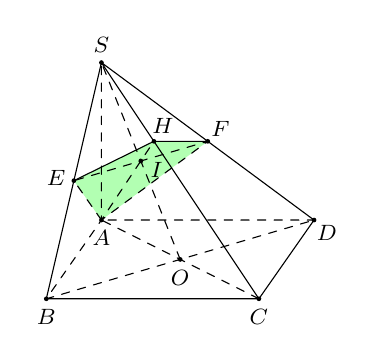
\begin{tikzpicture}[scale=1,>=stealth,font=\footnotesize,line join=round,line cap=round,declare function={h=2;}]
					 \path
						 (0,0) coordinate (A)
						(-0.7,-1) coordinate (B) 
						(2,-1) coordinate (C) 
						(barycentric  cs:A=1,C=1,B=-1) coordinate (D)
						(A)+(90:h) coordinate (S) 
						(barycentric cs:A=1,C=1) coordinate (O) 
						 (barycentric cs:S=2,C=1) coordinate (H)
						(intersection of  A--H and S--O) coordinate (I)
						(barycentric cs:I=3,D=1,O=-1) coordinate  (X)
						(intersection of S--B and I--X) coordinate  (E)
						 (intersection of S--D and I--X) coordinate (F);
					\fill[green!30] (A)--(E)--(H)--(F)--cycle; 
					 \draw[dashed] (O)--(S)--(A)--(B)--(D)
						(C)--(A)--(D) 
						(A)--(E)--(F)--(A)--(H); 
					\draw (C)--(S)--(B)--(C)--(D)--(S) 
						(E)--(H)--(F); 
					\foreach \p/\g  in{A/-90,B/-90,C/-90,D/-45,S/90,O/-90,H/60,I/-30,E/170,F/45}
					\fill (\p) circle (.03)  node[shift={(\g:.23)},scale=1]{$\p$};
				\end{tikzpicture}
		\end{center}
		Gọi $(\alpha)$ là mặt phẳng qua $A$ và vuông góc với $SC$.\\ 
		Gọi $H=(\alpha)\cap  SC$, suy ra $AH\perp SC$.\\
		 Gọi $E=(\alpha)\cap SB$, suy ra $EH\perp SC$.\\
		Gọi $F=(\alpha)\cap SD$, suy ra  $FH\perp SC$.\\
		Ta được tứ giác $AEHF$ là thiết diện của hình chóp $S. ABCD$ tạo  bởi mặt phẳng $(\alpha)$.\\
		Vì $\heva{&  BC\perp AB\\ & BC\perp SA}\Rightarrow BC\perp(SAB)\Rightarrow BC\perp AE$.\\
		 Mà $AE\perp SC$ nên $AE\perp(SBC)$.\\
		 Suy ra $\heva{& AE\perp SB\\ & AE\perp EH.}$\\
		Tương tự ta cũng có $\heva{&AF\perp  SD\\ &AF\perp FH.}$\\
		Ta có  $\triangle SAB=\triangle SAD\Rightarrow AE=AF\Rightarrow EH=FH\Rightarrow\triangle AEH=\triangle AFH$.\\
		Suy ra $S_{AEHF}=2S_{\triangle  AEH}=AE\cdot EH$.\\
		$AE=\dfrac{SA\cdot AB}{\sqrt{SA^2+AB^2}}=\dfrac{x}{\sqrt{1+x^2}}$,\\ 
		 $AH=\dfrac{SA\cdot AC}{\sqrt{SA^2+AC^2}}=\dfrac{x\sqrt{2}}{\sqrt{1+2 x^2}}$,\\
		$EH=\sqrt{AH^2-AE^2}=\sqrt{\dfrac{2  x^2}{1+2 x^2}-\dfrac{x^2}{1+x^2}}=\dfrac{x}{\sqrt{\left(1+2 2x^2\right)\left(1+2 x^2\right)}}$.\\
		Do đó,\allowdisplaybreaks 
		\begin{align*}
			 S_{AEHF}=\dfrac{x^2}{\sqrt{\left(1+2 x^2\right)\left(1+x^2\right)\left(1+x^2\right)}}
			=\dfrac{x^2}{\left(1+2 x^2\right)\sqrt{1+2  x^2}}.
		\end{align*}
		Theo  bất đẳng thức AM-GM, ta có $1+x^2\geq 2x$.\\
		 Theo bất đẳng thức Cauchy-Schwars, ta có $1+2x^2=\dfrac{1}{1}+\dfrac{x^2}{1}+\dfrac{x^2}{1}\geq\dfrac{(1+x+x)^2}{1+1+1}=\dfrac{(2x+1)^2}{3}$.\\
		 Do đó,
		\begin{align*}
			 S_{AEHF}&=\dfrac{x^2}{\left(1+2 x^2\right)\sqrt{1+2 x^2}}\\
			&\le\dfrac{x^2}{2x\cdot \dfrac{2x+1}{\sqrt{3}}}\\ 
			&=\dfrac{x\sqrt{3}}{2(x+x+1)}\\ 
			&\le\dfrac{x\sqrt{3}}{6\cdot  \sqrt[3]{x^2}}\\
			&=\dfrac{\sqrt{3}\cdot  \sqrt[3]{x}}{6}\le\dfrac{\sqrt{3}}{6}.
		\end{align*}
		Vậy $S_{AEHF}$ lớn nhất là $\dfrac{\sqrt{3}}{6}$  khi $x=1$.
	} 
\end{ex}

% nguồn: Ok_Toan11_TracNghiem_Lan2
\begin{ex}%[1H8V2-4]%[ma:3ea7607e]
	Cho hình chóp $S.ABC$ có đáy $ABC$ là tam giác đều và  $H$ là trung điểm cạnh $BC$. Gọi $O$ là trung điểm $AH$ của tam giác $ABC$, $SO$ vuông góc với đáy. Gọi $I$ là trung điểm $OH$. Mặt phẳng $(P)$ qua $I$ và vuông góc với $OH$. Thiết diện của $(P)$ và hình chóp $S.ABC$ là hình gì?
	 \choice
		{\True  Hình thang cân}
		 {Tam giác vuông}
		{Hình  thang vuông}
		{Hình  bình hành}
	\loigiai{ 
		\begin{center}
			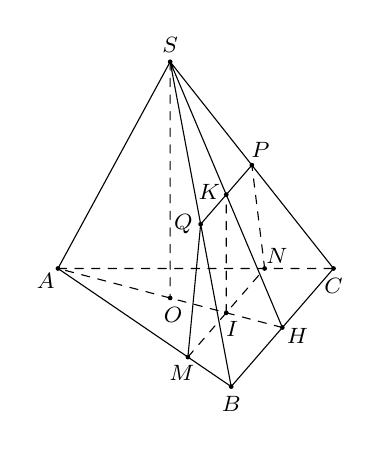
\begin{tikzpicture}[scale=1,>=stealth,font=\footnotesize,line join=round,line cap=round,declare function={h=3;}]
					\path 
						(0,0) coordinate (A) 
						 (2.2,-1.5) coordinate (B)
						(3.5,0) coordinate  (C)
						(barycentric cs:B=1,C=1) coordinate  (H)
						 (barycentric cs:A=1,H=1) coordinate (O)
						(O)+(90:h)  coordinate (S)
						(barycentric cs:O=1,H=1)  coordinate (I)
						(barycentric cs:I=1,C=1,H=-1) coordinate (x) 
						(intersection of A--B and  I--x) coordinate (M)
						(intersection of A--C  and I--x) coordinate (N)
						(barycentric cs:I=3,O=-1,S=1) coordinate (y) 
						(intersection of S--H and I--y) coordinate  (K)
						(barycentric cs:K=3,H=-1,B=1) coordinate (z) 
						(intersection of S--C and K--z)  coordinate (P)
						(intersection of S--B and K--z) coordinate (Q); 
					\draw[dashed] (S)--(O) 
						 (H)--(A)--(C)
						 (M)--(N)--(P)
						(I)--(K); 
					\draw (A)--(B)--(C)--(S)--(A) 
						(H)--(S)--(B) 
						 (M)--(Q)--(P);
					\foreach \p/\g in{A/-135,B/-90,C/-90,S/90,H/-30,O/-80,I/-70,M/-110,N/45,K/170,P/60,Q/180} 
					\fill (\p) circle  (.03) node[shift={(\g:.22)},scale=1]{$\p$};
				\end{tikzpicture}
		\end{center}
		Ta có  $\heva{&(P)\perp OH\\ &BC\perp OH}\Rightarrow(P)\parallel BC$.\\
		Qua $I$ kẻ đường thẳng $d_1$  song song với $BC$. Gọi $\heva{&d_1\cap AB=M\\ &d_1\cap AC=N.}$\\
		Ta  có $\heva{&SO\perp OH\\ &(P)\perp OH}\Rightarrow(P)\parallel SO$.\\
		Qua $I$ kẻ đường thẳng $IK$  song song với $SO$ $(K\in SH)$.\\
		$(P)\parallel BC$. Qua $K$ kẻ  đường thẳng $d_2\parallel BC$. Gọi $\heva{& d_2\cap SB=Q\\ & d_2\cap SC=P.}$\\
		Do đó, thiết diện của $(P)$ và hình chóp  $S. ABC$ là tứ giác $MNPQ$ có $IK$ là đường trung trực của $MN$ và $PQ$.\\
		 Vậy $MNPQ$ là hình thang cân.
	} 
\end{ex}


%%%%%%%%%%%%%%%% TRẢ LỜI NGẮN %%%%%%%%%%%%%%%%

% nguồn: Ok_TraLoiNgan_Lop11_Lan1
\begin{ex}%[1H8V2-4]%[ma:2d2bf781]
	Cho hình chóp $S.ABCD$ có đáy $ABCD$ là  hình vuông tâm $O$ cạnh $a$, $SA=a\sqrt{6}$ và $SA$ vuông góc mặt phẳng $(ABCD)$. Gọi $H, K$ lần lượt là chân đường cao hạ từ đỉnh $A$ của các tam giác $SAB$ và $SAD$. Thiết diện của hình chóp khi cắt bởi mặt phẳng $(AHK)$ bằng
	$\dfrac{b\cdot a^2\sqrt{3}}{c}$, với $\dfrac{b}{c}$, $b\in\mathbb{N}$ và $c\in\mathbb{Z}$, là phân số tối  giản. Tính $b+c$.
	 \shortans{10}
	\loigiai{ 
		\begin{center}
			\begin{tikzpicture}[scale=1,font=\footnotesize,line join=round,line cap=round,>=stealth]
					\path (0:0) coordinate  (A)++(0:4) coordinate (D)++(-120:2) coordinate (C) ++(180:4) coordinate (B)
						(A)++(90:3) coordinate (S) 
						 ($(A)!.5!(C)$) coordinate (O)
						($(S)!.8!(B)$)  coordinate (H)
						($(S)!.8!(D)$) coordinate  (K)
						($(H)!.5!(K)$)  coordinate (I)
						(intersection of A--I and S--C) coordinate (J); 
					 \draw[dashed] (S)--(A)--(B)--(D)--(A)--(C)
						(A)--(J) 
						(A)--(H)--(K)--(A) 
						(S)--(O); 
					\draw  (S)--(B)--(C)--(S)--(D)--(C)
						 (H)--(J)--(K);
					\foreach \x/\g in {S/90,A/150,B/-90,C/-90,D/0,O/90,H/180,J/-30,K/70,I/-135} \fill (\x) circle (1pt)+(\g:.25) node {$\x$}; 
				\end{tikzpicture}
		\end{center}
		\begin{itemize}
			\item Ta có $\left(SC,(ABCD)\right)=(SC,AC)=\widehat{SCA}$ và 
			$\tan\widehat{SCA}=\dfrac{SA}{AC}=\sqrt{3}$ nên  $\left(SC,(ABCD)\right)=60^{\circ}$.
			\item  Vì $AH \perp SB$ và $AH\perp BC$ nên $AH \perp SC$. Tương tự $AK\perp SC$. Do đó $SC\perp (AHK)$.
			\item Gọi $I$  là giao điểm của $HK$ và $SO$, $J$ là giao điểm của $AI$ và $SC$.\\
			Thiết diện  cần tìm là tứ giác $AHJK$.\\
			Ta có $AH=\dfrac{SA\cdot AB}{SB}=\dfrac{a\sqrt{42}}{7}$ và $AH\perp (SBC)$ nên $AH  \perp HJ$.\\
			Tương tự $AK \perp KJ$  và $AK=\dfrac{a\sqrt{42}}{7}$.\\
			Từ đó suy ra hai tam giác vuông $AHJ$ và $SKJ$  bằng nhau, do đó $$S_{AHJK}=S_{AHJ}+S_{AKJ}=2S_{AHJ}.$$
			 Ta có $SH^2=SA^2-AH^2 \Rightarrow SH=\dfrac{6a\sqrt{7}}{7}$.\\
			Vì $SC\perp (AHK)$ nên $SC\perp HJ$, do đó tam giác $SHJ$ vuông tại $J$. Suy ra hai tam giác vuông $SBC$ và $SJH$ đồng dạng nên $$\dfrac{JH}{BC}=\dfrac{SH}{SC} \Rightarrow JH=\dfrac{SH\cdot  BC}{SC}=\dfrac{3a\sqrt{14}}{14}.$$
			Vậy $S_{AHJK}=2S_{AHJ}=AH\cdot  JH=\dfrac{3a^2\sqrt{3}}{7}$.
		\end{itemize}
	 }
\end{ex}


%%%%%%%%%%%%%%%% TỰ LUẬN %%%%%%%%%%%%%%%%

% nguồn: Ok_TuanLuan_Toan11_Lan2
\begin{ex}%[1H8H2-4]%[ma:439dec85]
	Cho hình chóp $S.ABC$ có đáy $ABC$ là tam giác vuông cân tại $A$, $AB=AC=a$; cạnh bên $SA$ vuông góc với mặt đáy, $SA=a$. Gọi $M$ là trung điểm của $SC$. Tính diện tích thiết diện của hình chóp cắt bởi mặt phẳng $(P)$ đi qua $M$  và vuông góc với $AC$.
	\loigiai{ 
	 \immini{
		Gọi $E$, $F$ lần lượt là trung điểm  của $AC$, $BC$.\\
		Do đó $ME\parallel SA$, $EF\parallel  AB$ (tính chất đường trung bình trong tam giác).\\
		Mà $SA\perp (ABC)$ (gỉả thiết) nên $ME\perp (ABC)$, suy ra  $ME\perp EF$.\\
		Dễ thấy $(MEF)\equiv (P)$, thiết diện là tam giác $MEF$ vuông  tại $E$.\\
		Vậy diện tích thiết diện là 
		$$S=\dfrac{1}{2}ME\cdot EF=\dfrac{1}{2}\cdot\dfrac{1}{2}SA\cdot\dfrac{1}{2}AB =\dfrac{a^2}{8}.$$ 
		}{ 
		\begin{tikzpicture}[scale=0.8,font=\footnotesize,line join=round,line cap=round,>=stealth]
				\def\ac{4} 
				\def\ba{2} 
				\def\h{3.5} 
				 \def\gocA{-45}
				\coordinate[label=left:$A$] (A)  at (0,0);
				\coordinate[label=below:$B$] (B) at (\gocA:\ba); 
				\coordinate[label=right:$C$] (C) at (\ac,0); 
				\coordinate[label=above:$S$] (S) at  ($(A)+(90:\h)$);
				\coordinate[label=above:$M$] (M) at  ($(S)!0.5!(C)$);
				\coordinate[label=below left:$E$]  (E) at ($(A)!0.5!(C)$);
				\coordinate[label=below right:$F$] (F) at ($(B)!0.5!(C)$); 
				\draw  (S)--(A)--(B)--(C)--cycle (S)--(B)
					(M)--(F); 
				 \draw[dashed] (A)--(C)
					(M)--(E)--(F); 
				\foreach \diem in  {A,B,C,S,M,E,F} \fill (\diem) circle (1pt);
			\end{tikzpicture}
		 }
	} 
\end{ex}

% nguồn: Ok_TuanLuan_Toan11_Lan1
\begin{bt}%[1H8V2-4]%[ma:f9c684ea]
	Cho hình chóp $S.ABC$ có đáy $ABC$ là tam giác vuông tại $B$, các cạnh $AB=3$, $BC=2$, cạnh bên $SA=2$ và $SA$ vuông góc với đáy. Mặt phẳng $(\alpha)$ qua $A$, vuông góc $SB$ cắt $SB$ và $SC$ lần lượt tại $M$ và $N$. Diện tích của tam giác $AMN$ bằng bao nhiêu? (Làm tròn kết  quả đến $2$ chữ số sau dấu phấy).
	\loigiai{ 
	 \immini
		{Dễ thấy $AM\perp (SBC)$  và\\
		$AM=\dfrac{AS\cdot AB}{\sqrt{AS^2+AB^2}}=\dfrac{2\cdot  3}{\sqrt{2^2+3^2}}=\dfrac{6\sqrt{13}}{3}$.\\
		Ta có $MN$ và $BC$ cùng vuông góc $SB$ nên song song nhau, từ đó  $\dfrac{MN}{BC}=\dfrac{SM}{SB}=\dfrac{SA^2}{SB^2}=\dfrac{4}{13}$.\\
		Suy ra  $MN=BC\cdot \dfrac{4}{13}=\dfrac{8}{13}$.\\
		Tam giác $AMN$  vuông tại $M$ nên có diện tích là $$\mathrm{S}=\dfrac{1}{2}\cdot \dfrac{6\sqrt{13}}{13}\cdot \dfrac{8}{13}=0,51 (\text{Đvtt}).$$}
		{\begin{tikzpicture}[>=stealth,line join=round,line cap=round,font=\footnotesize,scale=0.6]
		 \path
			(0,0)  coordinate (A)
			(3,-3) coordinate  (B)
			(8,0)  coordinate (C)
			 (0,5) coordinate (S)
			($(S)!.4!(B)$) coordinate (M) 
			($(S)!.4!(C)$) coordinate (N); 
		\draw (S)--(B)--(C)--(S)--(A)--(B) 
			 (A)--(M)--(N);
		\draw[dashed]  (A)--(C)
			(A)--(N); 
		\foreach \x/\g in {A/160,B/-60,C/-60,S/90,M/180,N/60}\fill (\x) circle (1.5pt)+(\g:3mm) node{$ \x $}; 
	\end{tikzpicture}
		 }
	 }
\end{bt}

% nguồn: Ok_TuanLuan_Toan11_Lan2
\begin{ex}%[1H8V2-4]%[ma:f6adf02d]
	Cho hình chóp $S.ABC$ có đáy $ABC$ là tam  giác vuông tại $B$, các cạnh $AB=3$, $BC=2$, cạnh bên $SA=2$ và $SA$ vuông góc với đáy. Mặt phẳng $(\alpha)$ qua $A$, vuông góc $SB$ cắt $SB$ và $SC$ lần lượt tại $M$ và $N$. Diện tích của tam giác $AMN$ bằng bao nhiêu? (Làm tròn kết quả đến $2$ chữ số sau dấu phấy).
	 \loigiai{
	\immini 
		{Dễ thấy $AM\perp (SBC)$ và\\ 
		 $AM=\dfrac{AS\cdot AB}{\sqrt{AS^2+AB^2}}=\dfrac{2\cdot 3}{\sqrt{2^2+3^2}}=\dfrac{6\sqrt{13}}{3}$.\\
		Ta có $MN$ và $BC$ cùng vuông góc $SB$ nên song song nhau, từ đó $\dfrac{MN}{BC}=\dfrac{SM}{SB}=\dfrac{SA^2}{SB^2}=\dfrac{4}{13}$.\\ 
		 Suy ra $MN=BC\cdot \dfrac{4}{13}=\dfrac{8}{13}$.\\
		Tam giác $AMN$ vuông tại $M$ nên có diện tích là $$\mathrm{S}=\dfrac{1}{2}\cdot  \dfrac{6\sqrt{13}}{13}\cdot \dfrac{8}{13}=0,51 (\text{Đvtt}).$$}
		{\begin{tikzpicture}[>=stealth,line join=round,line cap=round,font=\footnotesize,scale=0.6]
		\path 
			(0,0) coordinate (A) 
			(3,-3) coordinate  (B)
			(8,0) coordinate (C) 
			(0,5) coordinate  (S)
			($(S)!.4!(B)$)  coordinate (M)
			($(S)!.4!(C)$)  coordinate (N);
		\draw (S)--(B)--(C)--(S)--(A)--(B) 
			 (A)--(M)--(N);
		 \draw[dashed] (A)--(C)
			(A)--(N); 
		\foreach \x/\g in {A/160,B/-60,C/-60,S/90,M/180,N/60}\fill  (\x) circle (1.5pt)+(\g:3mm) node{$ \x $};
	\end{tikzpicture}
		 }
	 }
\end{ex}

% nguồn: Ok_TuanLuan_Toan11_Lan2
\begin{ex}%[1H8V2-4]%[ma:c51ea1da]
	Cho hình chóp $S.ABCD$ với đáy $ABCD$ là hình  thang vuông tại $A$, đáy lớn $AD=8$, đáy nhỏ $BC=6$, $SA$ vuông góc với đáy, $SA=6$. Gọi $M$ là trung điểm của $AB$, $(P)$ là mặt phẳng qua $M$ và vuông góc với $AB$. Thiết diện của hình chóp $S.ABCD$ cắt bởi mặt phẳng $(P)$ có diện tích bằng bao nhiêu?
	 \loigiai{
	 \immini{
		Gọi $N$, $P$ và $Q$ lần lượt là trung điểm của $CD$,  $SC$ và $SB$.\\
		Ta có $\heva{& (P)\cap(SAB)=MQ\\& (P)\cap(ABCD)=MN\\& (P)\cap(SCD)=NP.}$\\ 
		Do đó, thiết diện của hình chóp  $S.ABCD$ cắt bởi mặt phẳng $(P)$ là tứ giác $MNPQ$.\\
		Khi đó $MNPQ$ là hình thang vuông tại $M$, $Q$ và $MQ=PQ=3$,  $MN=7$.
		}{ 
		\begin{tikzpicture}[scale=0.8,font=\footnotesize,line join=round,line cap=round,>=stealth]
				 \def\bc{2}
				\def\ba{2.2} 
				 \def\ad{5}
				\def\h{3.5} 
				\def\gocB{140} 
				\coordinate[label=below:$B$] (B) at (0,0); 
				\coordinate[label=left:$A$]  (A) at (\gocB:\ba);
				\coordinate[label=below:$C$]  (C) at (\bc,0);
				\coordinate[label=right:$D$]  (D) at ($(A)+(0:\ad)$);
				\coordinate[label=above:$S$] (S) at ($(A)+(90:\h)$); 
				\coordinate[label=below  left:$M$] (M) at ($(A)!0.5!(B)$);
				\coordinate[label=below right:$N$]  (N) at ($(C)!0.5!(D)$);
				\coordinate[label=above:$P$] (P) at ($(S)!0.5!(C)$); 
				 \coordinate[label=left:$Q$] (Q) at ($(S)!0.5!(B)$);
				\draw  (S)--(A)--(B)--(C)--(D)--cycle (B)--(S)--(C)
					(M)--(Q)--(P)--(N); 
				\draw[dashed] (A)--(D) 
					 (M)--(N);
				\foreach \diem in {A,B,C,D,S,M,N,P,Q}  \fill (\diem) circle (1pt);
			\end{tikzpicture}
		 }
		\noindent 
		Vậy diện tích hình thang  $MNPQ$ là $$S_{MNPQ}=\dfrac{MQ\cdot (MN+PQ)}{2}=\dfrac{3\cdot (7+3)}{2}=15.$$
	} 
\end{ex}

% nguồn: Ok_TuanLuan_Toan11_Lan2
\begin{ex}%[1H8V2-4]%[ma:c922adf2]
	Cho hình chóp $S.ABCD$ có đáy $ABCD$ là hình vuông cạnh $a$, cạnh bên $SA=b$ và vuông góc với  mặt phẳng đáy $(ABCD)$. Gọi $M$ là điểm trên cạnh $AB$ sao cho $AM=x$ ($0<x<a$). Gọi $(\alpha)$ là mặt phẳng qua $M$ vuông góc với đường thẳng $AC$.
	\begin{enumerate}
		\item Xác định thiết diện của hình chóp đã cho với mặt phẳng  $(\alpha)$.
		\item Tính diện tích $S$ của thiết diện theo  $a$, $b$, $x$.
		\item Tìm $x$ để diện tích của thiết  diện lớn nhất.
	\end{enumerate}
	\loigiai{ 
		\begin{center}
			\begin{tikzpicture}[>=stealth,line join=round,line cap=round,font=\footnotesize,scale=1]
					 \tikzset{
						pics/hinhChopTuGiac/.style n  args={5}{
						code={ 
					 \tikzset{
						declare  function={a=5; b=2; h=3.5; goc=-130;}
					} 
					\path 
						 (0,0) coordinate (#1)+(0:a) coordinate (#2)+(goc:b) coordinate (#4)+(90:h) coordinate (#5)
						($(#2)+(#4)-(#1)$)  coordinate (#3);
					\foreach \pointo/\pointt in {#1/#2,#1/#5,#1/#4}{ 
						\draw[fill,dashed](\pointo)--(\pointt); 
					} 
					\foreach \pointo/\pointt  in {#5/#2,#5/#4,#5/#3,#3/#2,#3/#4}{
						\draw (\pointo)--(\pointt); 
					 }
					} 
						}} 
					 \tikzset{declare function={ratio=.4;}}
					 \path
						(0,0) pic  {hinhChopTuGiac={A}{B}{C}{D}{S}}
						($(A)!ratio!(B)$) coordinate (M) 
						($(A)!ratio!(D)$) coordinate  (L)
						($(S)!ratio!(B)$) coordinate (N) 
						 ($(S)!ratio!(D)$) coordinate (Q)
						(intersection of  M--L and A--C) coordinate (I)
						($(I)+(S)-(A)$)  coordinate (t)
						(intersection of S--C and  I--t) coordinate (P)
						(intersection of A--C  and B--D) coordinate (O);
					\foreach \pointo/\pointt in {P/N,Q/P}{ 
						 \draw[fill](\pointo)--(\pointt);
					 }
					 \fill[opacity=.2]
						(P)--(N)--(M)--(L)--(Q)--cycle; 
					\foreach  \pointo/\pointt in {A/C,B/D,N/M,M/L,L/Q,I/P}{
						\draw[fill,dashed](\pointo)--(\pointt); 
					 }
					\foreach \point/\goc  in {S/90,A/170,B/0,D/220,C/-20,O/-90,P/90,N/70,M/30,Q/160,L/180,I/-100}{
						\draw[fill](\point)  circle (.8pt)+(\goc:2.5mm) node[scale=.8]{$\point$};
					 }
				\end{tikzpicture}
		\end{center}
		\begin{enumerate}
			\item Xác định  thiết diện của hình chóp đã cho với mặt phẳng $(\alpha)$.\\
			Ta có $\heva{&SA \perp AC \\  &BD \perp AC}
			$,  suy ra $(\alpha) \parallel SA$ và $(\alpha) \parallel BD$.
			\begin{enumerate}
				\item $\heva{&(\alpha) \parallel SA \\ &SA \subset (SAB)} \Rightarrow (\alpha) \cap (SAB) = m$ với $m$ đi qua $M$ và song song với $SA$, cắt cạnh $SB$ tại $N$. 
				\item $\heva{&(\alpha)  \parallel BD \\ &BD \subset (ABCD)} \Rightarrow (\alpha) \cap (ABCD) = n$, với $n$ đi qua $M$ và song song với $BD$, cắt cạnh $AD$ tại $L$ và cắt đoạn $AC$ tại $I$.
				\item $\heva{&(\alpha) \parallel SA \\ &SA \subset (SAC)} \Rightarrow (\alpha) \cap (SAC) = p$, với $p$ đi qua $I$ và song  song với $SA$, cắt cạnh $SC$ tại $P$.
				\item $\heva{&(\alpha) \parallel SA \\ &SA \subset (SAD)} \Rightarrow  (\alpha) \cap (SAD) = q$, với $q$ đi qua $L$ và song song với $SA$, cắt cạnh $SD$ tại $Q$.
			\end{enumerate}
			Mặt phẳng $(\alpha)$ cắt các mặt  của hình chóp $S.ABCD$ theo năm đoạn giao tuyến $MN$, $NP$, $PQ$, $QL$, $LM$, nên thiết diện là ngũ giác $MNPQL$.
			\item Tính diện tích $S$ của thiết diện theo $a$, $b$, $x$.\\ 
			Chú ý tính chất  đối xứng ta có $S_{MNPQL} = 2S_{MINP}$.\\
			Trong đó tứ giác $MINP$ là hình  thang vuông tại $I$ và $M$, gọi $O$ là tâm hình vuông $ABCD$ ta có theo định lí Ta-lét, ta có
			 \allowdisplaybreaks
			\begin{eqnarray*}
				 &&\dfrac{MN}{SA} = \dfrac{BM}{BA} = \dfrac{a-x}{a} \Rightarrow MN=\dfrac{b(a-x)}{a},\\[5pt]
				&&\dfrac{MI}{BO} = \dfrac{AM}{AB} = \dfrac{x}{a}  \Rightarrow MI=\dfrac{x\sqrt{2}}{2},\\[5pt]
				&&\dfrac{IP}{SA} = \dfrac{CI}{CA}  = \dfrac{CO+OI}{2OA} = \dfrac{1}{2}+\dfrac{OI}{2OA}
				= \dfrac{1}{2}+\dfrac{BM}{2BA} = \dfrac{1}{2}+\dfrac{a-x}{2a} =  \dfrac{2a-x}{2a}.
			\end{eqnarray*}
			Suy ra $IP=\dfrac{b(2a-x)}{2a}$.\\ 
			Khi  đó
			\[S_{MNPQL}=(MN+IP)MI=\left[\dfrac{b(a-x)}{a}+\dfrac{b(2a-x)}{2a}\right]\dfrac{x\sqrt{2}}{2}=\dfrac{\sqrt{2}bx(4a-3x)}{4a}.\] 
			\item Tìm $x$ để diện tích của  thiết diện lớn nhất.\\
			Sử dụng bất  đẳng thức Cô-si ta có
			\[S=\dfrac{\sqrt{2}bx(4a-3x)}{4a}=\dfrac{\sqrt{2}b}{12a}\cdot  3x(4a-3x)\le\dfrac{\sqrt{2}b}{12a}\left(\dfrac{3x+4a-3x}{2}\right)^{2}=\dfrac{\sqrt{2}ab}{3}.\]
			Dấu \lq\lq=\rq\rq\,  xảy ra khi $3x = 4a-3x \Leftrightarrow x = \dfrac{2a}{3}$.
		\end{enumerate}
	 }
\end{ex}

% nguồn: Ok_TuanLuan_Toan11_Lan2
\begin{ex}%[1H8V2-4]%[ma:b9542bd4]
	Cho hình chóp $S.ABC$ có đáy $ABC$ là tam giác vuông tại $B$ với $AB=a$, $BC=a\sqrt{3}$, cạnh bên $SA=a\sqrt{3}$ và vuông góc với mặt phẳng $(ABC)$. Mặt phẳng $(P)$ đi qua trung  điểm $M$ của $AB$ và vuông góc với $SB$ cắt $AC$, $SC$, $SB$ lần lượt tại $N$, $P$, $Q$. Diện tích của tứ giác $MNPQ$ bằng bao nhiêu?
	\loigiai{ 
	 \immini{
		Ta có  $BC\perp (SAB) \Rightarrow BC\perp SB$.\\
		Do mặt phẳng $(P)$ đi qua trung điểm  $M$ của $AB$ và vuông góc với $SB$ cắt $AC$, $SC$, $SB$ lần lượt tại $N$, $P$, $Q$ nên $MN\parallel PQ\parallel BC$.\\
		Nên  tứ giác $MNPQ$ là hình thang vuông tại $M$, $Q$.\\
		Khi đó  $S_{MNPQ}=\dfrac{1}{2}(MN+PQ)\cdot MQ$.
		\begin{itemize}
			\item Xét $\triangle ABC$ có $MN\parallel BC$, $MN=\dfrac{1}{2}BC =\dfrac{a\sqrt{3}}{2}$. 
			\item Xét $\triangle MQB \backsim \triangle SAB$ ta có $\dfrac{MQ}{MB}=\dfrac{SA}{SB}$. 
			$$\Rightarrow MQ=\dfrac{SA\cdot MB}{SB}  =\dfrac{a\sqrt{3}\cdot a}{2a\cdot 2}=\dfrac{a\sqrt{3}}{4}.$$
			Suy ra  $QB=\sqrt{MB^2-MQ^2}=\dfrac{a}{4}$.\\
			Xét  $\triangle SAB$ có $SB=\sqrt{SA^2+AB^2}=2a$.\\
			$\Rightarrow  SQ=SB-QB=\dfrac{7a}{4}$.
		\end{itemize}
		}{ 
		\begin{tikzpicture}[scale=0.8,font=\footnotesize,line join=round,line cap=round,>=stealth]
				 \def\ac{5}
				 \def\ba{2.2}
				\def\h{3.5} 
				 \def\gocA{-45}
				\coordinate[label=left:$A$] (A) at (0,0); 
				\coordinate[label=below:$B$] (B)  at (\gocA:\ba);
				\coordinate[label=right:$C$] (C)  at (\ac,0);
				 \coordinate[label=above:$S$] (S) at ($(A)+(90:\h)$);
				\coordinate[label=below  left:$M$] (M) at ($(A)!0.5!(B)$);
				\coordinate[label=below:$N$] (N)  at ($(A)!0.5!(C)$);
				\coordinate[label=above:$P$] (P) at ($(S)!0.6!(C)$); 
				\coordinate[label=left:$Q$] (Q)  at ($(S)!0.6!(B)$);
				\draw  (S)--(A)--(B)--(C)--cycle (S)--(B)
					(M)--(Q)--(P); 
				 \draw[dashed] (A)--(C)
					 (M)--(N)--(P);
				\foreach \diem  in {A,B,C,S,M,N,P,Q} \fill (\diem) circle (1pt);
			\end{tikzpicture}
		} 
		 \noindent
		\begin{itemize}
			\item Lại có $MN\parallel PQ\parallel BC$  nên $\dfrac{PQ}{BC}=\dfrac{SQ}{SB}$.\\
			 $\Rightarrow PQ=\dfrac{SQ\cdot BC}{SB}=\dfrac{7a\sqrt{3}}{8}$.
		\end{itemize}
		Vậy $S_{MNPQ}=\dfrac{1}{2}(MN+PQ)\cdot  MQ=\dfrac{33a^2}{64}$.
	 }
\end{ex}

% nguồn: Ok_TuanLuan_Toan11_Lan2
\begin{ex}%[1H8V2-4]%[ma:be7fb9cd]
	Cho hình chóp $S.ABC$ có đáy $ABC$ là tam giác đều cạnh $a$, $SA=a$ và vuông góc với đáy. Mặt phẳng $(\alpha)$ qua $A$ và vuông góc với trung tuyến $SI$ của tam giác $SBC$. Tính diện tích $S$ của thiết diện tạo bởi $(\alpha)$  với hình chóp đã cho.
	\loigiai{ 
	 \immini{
		Gọi $H$ là  hình chiếu vuông góc của $A$ lên $SI$.\\
		Kẻ đường thẳng $MN$ qua $H$ và song song với $BC$ và  cắt $SB$, $SC$ lần lượt tại $M$, $N$.\\
		Ta có $SI\perp BC\Rightarrow SI\perp MN$ và  $SI \perp AH$.\\
		$\Rightarrow SI \perp  (AMN)$.\\
		 Lại có $\heva{& BC\perp SA\\& BC\perp AI} \Rightarrow BC\perp (SAI)$\\
		$\Rightarrow AH\perp BC \Rightarrow AH\perp MN$.\\ 
		 Xét $\triangle ABC$ đều có $AI=\dfrac{a\sqrt{3}}{2}$.\\
		Suy ra $AH=\sqrt{\dfrac{SA^2\cdot AI^2}{SA^2+AI^2}} = \dfrac{\sqrt{21}}{7}a$. 
		}{ 
		\begin{tikzpicture}[scale=1,font=\footnotesize,line join=round,line cap=round,>=stealth]
				 \def\ac{5}
				\def\ba{4} 
				\def\h{3.5} 
				\def\gocA{-30} 
				\coordinate[label=left:$A$] (A) at (0,0); 
				\coordinate[label=below:$B$] (B) at  (\gocA:\ba);
				\coordinate[label=right:$C$] (C) at (\ac,0); 
				\coordinate[label=above:$S$] (S)  at ($(A)+(90:\h)$);
				\coordinate[label=below right:$I$] (I)  at ($(B)!0.5!(C)$);
				\coordinate[label=right:$M$] (M)  at ($(S)!0.6!(B)$);
				\coordinate[label=above right:$N$] (N) at ($(S)!0.6!(C)$); 
				 \coordinate[label=right:$H$] (H) at ($(S)!0.6!(I)$);
				\draw (S)--(A)--(B)--(C)--cycle  (I)--(S)--(B)
					 (A)--(M)--(N);
				\draw[dashed] (I)--(A)--(C) 
					(N)--(A)--(H); 
				\foreach \diem in {A,B,C,S,I,M,N,H}  \fill (\diem) circle (1pt);
			\end{tikzpicture}
		} 
		 \noindent
		Ta  có $SI = \sqrt{SA^2 + AI^2} = \dfrac{\sqrt{7}}{2}a$.\\
		Do đó  $SA^2=SI\cdot SH\Rightarrow SH=\dfrac{2}{\sqrt{7}}a$.\\
		Mà $MN\parallel BC\Rightarrow  \dfrac{MN}{BC}=\dfrac{SH}{SI}\Rightarrow MN=\dfrac{4}{7}a$.\\
		 Vậy $S_{AMN}=\dfrac{1}{2}MN\cdot AH=\dfrac{2a^2\sqrt{21}}{49}$.
	} 
\end{ex}

% nguồn: Ok_TuanLuan_Toan11_Lan2
\begin{ex}%[1H8V2-4]%[ma:a146e58c]
	Cho hình chóp $S.ABCD$ có $SA$ vuông góc với đáy, $ABCD$ là hình vuông cạnh $a\sqrt{2}$, $SA=2a$. Gọi $M$ là trung điểm  của cạnh $SC$, $(\alpha)$ là mặt phẳng đi qua $A$, $M$ và song song với đường thẳng $BD$. Tính diện tích thiết diện của hình chóp $S.ABCD$ bị cắt bởi mặt phẳng $(\alpha)$.
	 \loigiai{
	 \immini{
		Gọi  $O=AC\cap BD$; $I=SO\cap AM$.\\
		Vì $(\alpha)$ là mặt phẳng đi qua $A$, $M$ và song song với đường thẳng $BD$ nên $(\alpha)$ cắt $(SBD)$ theo giao tuyến $PQ$  qua $I$ và $PQ\parallel BD$.\\
		Khi đó thiết diện của hình chóp $S.ABCD$ bị cắt  bởi mặt phẳng $(\alpha)$ là tứ giác $APMQ$.\\
		Ta có  $AC=BD=AB\sqrt{2}=a\sqrt{2}\cdot \sqrt{2}=2a$.\\
		Vì $\triangle SAC$ vuông tại $A$ và có  $M$ là trung điểm của cạnh $SC$ nên
		$$AM=\dfrac{1}{2}SC=\dfrac{1}{2}\cdot \sqrt{SA^2+AC^2}=a\sqrt{2}.$$ 
		}{ 
		\begin{tikzpicture}[scale=0.7,font=\footnotesize,line join=round,line cap=round,>=stealth]
				\def\bc{5} 
				\def\ba{2.2} 
				\def\h{4} 
				 \def\gocB{45}
				 \coordinate[label=below:$B$] (B) at (0,0);
				\coordinate[label=below:$A$] (A) at (\gocB:\ba); 
				\coordinate[label=below:$C$]  (C) at (\bc,0);
				\coordinate[label=right:$D$] (D)  at ($(A)+(0:\bc)$);
				\coordinate[label=above:$S$] (S) at  ($(A)+(90:\h)$);
				\coordinate[label=below:$O$]  (O) at ($(A)!0.5!(C)$);
				\coordinate[label=above right:$M$] (M) at  ($(S)!0.5!(C)$);
				\coordinate[label=left:$P$] (P)  at ($(S)!2/3!(B)$);
				\coordinate[label=right:$Q$] (Q) at  ($(S)!2/3!(D)$);
				\coordinate[label=above left:$I$] (I) at  ($(S)!2/3!(O)$);
				\draw  (S)--(B)--(C)--(D)--cycle (S)--(C)
					(P)--(M)--(Q); 
				\draw[dashed]  (B)--(A)--(D)--cycle (O)--(S)--(A)--(C)
					 (P)--(A)--(Q)--cycle (A)--(M);
				\foreach \diem  in {A,B,C,D,S,O,M,P,Q,I} \fill (\diem) circle (1pt);
			\end{tikzpicture}
		} 
		\noindent 
		Ta  có $SA$ vuông góc với đáy và $ABCD$ là hình vuông nên $BD\perp (SAC)$.\\
		$\Rightarrow PQ\perp (SAC)  \Rightarrow PQ\perp AM$.\\
		Vì $I$ là giao điểm hai đường trung tuyến  $SO$ và $AM$ của $\triangle SAC$ nên
		$$\dfrac{SI}{SO}=\dfrac{PQ}{BD}=\dfrac{2}{3}  \Rightarrow PQ=\dfrac{2}{3}BD=\dfrac{4}{3}a.$$
		Do  đó diện tích tứ giác $APMQ$ là
		$$S_{APMQ}=\dfrac{1}{2}PQ\cdot AM=\dfrac{1}{2}\cdot \dfrac{4}{3}a\cdot a\sqrt{2}=\dfrac{2a^2\sqrt{2}}{3}.$$ 
	} 
\end{ex}
